\section{Advanced concepts for VAEs with hands-on example}

This section marks the beginning of the advanced module in Machine Learning, which will cover several cutting-edge topics. We will begin with Generative Modeling, specifically exploring in more detail Variational Autoencoders and Normalizing Flows, which are currently among the most powerful and trendy generative techniques. We will then transition into advanced concepts for Graph Neural Networks and Transformer models with some realistic use cases.

\subsection{Recap of standard autoencoders}
To deeply understand modern generative models, let us first revisit the standard autoencoder. \\
An autoencoder consists of two distinct MLPs, as shown in figure:
\begin{itemize}
    \item[-] The encoder ($g_\phi$): Parameterized by weights $\phi$, it translates the original high-dimensional input $x$ (like an unwrapped $32 \times 32$ image) into a low-dimensional latent representation $z$.
    \item[-] The decoder ($f_\theta$): Parameterized by weights $\theta$, it takes the compressed code $z$ and attempts to reconstruct the original high-dimensional data as $x'$.
\end{itemize}

\begin{center}
    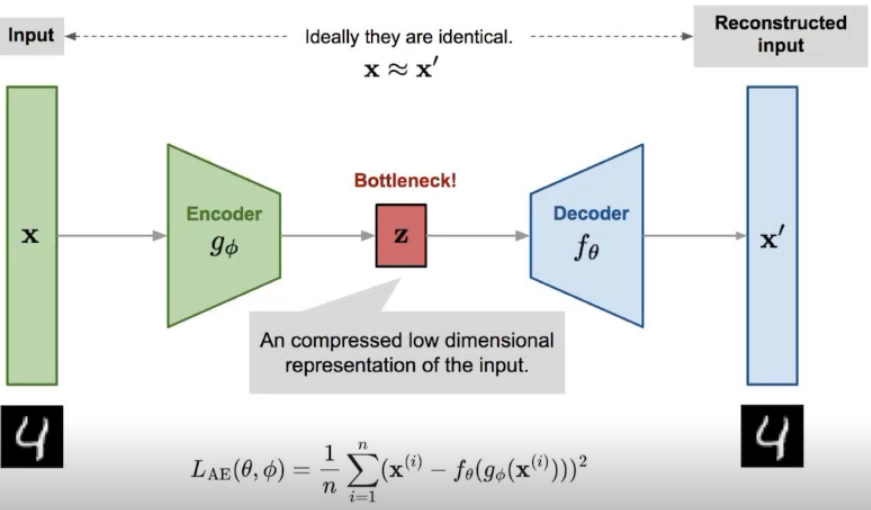
\includegraphics[width=0.6\textwidth]{figuresML_adv/lesson_ml_adv_1_pag_2.png}
\end{center}

An autoencoder is a neural network trained in an entirely unsupervised manner, since there are no explicit labels (e.g., "this is a dog" or "this is a cat"). The goal of the network is simply to reproduce its input, outputting a vector $x'$ as similar as possible to the input $x$. Due to the dimensionality reduction step, the output should looked "blurred" (if you think about an image) with respect to the input.

The critical feature of this architecture is the bottleneck: by forcing the data through a latent space $Z$ with a much smaller dimensionality than $X$, the network cannot simply learn the identity function, but it is forced to learn an efficient compression scheme, extracting the most vital underlying features of the data. The network is trained by minimizing a reconstruction loss, typically the mean squared error, between the input and the output:
\begin{equation}
    \mathcal{L}_{AE}(\theta, \phi) = \frac{1}{n} \sum_{i=1}^n \left( x^{(i)} - f_\theta(g_\phi(x^{(i)})) \right)^2
\end{equation}

While standard autoencoders are excellent for tasks like data compression or anomaly detection (e.g., fraud detection in finance), they \textit{cannot be used for generation}, because the latent space $Z$ is entirely unregularized. The encoder maps inputs to specific, isolated discrete points in the latent space, and if we arbitrarily sample a random point in an empty region of this latent space and pass it to the decoder, the network will output meaningless noise, as it has never learned what that empty space represents \footnote{This is actually the reason why autoencoders are useful for anomaly detection: a random point in the $Z$ space will be easily recognizable since it will most likely be projected far away from know clustered regions in the $X$ space by the network.}. 

\subsection{Variational Autoencoders in depth}

To transform the standard autoencoder into a true generative model, we must introduce stochasticity and regularize the latent space. We no longer want to map the input to a single, deterministic point; instead, we want to map it to a \textit{probability distribution}. This is the foundational concept of the Variational Autoencoder (VAE) and the very meaning behind the word "variational": running the inference process twice on the same input will yield similar, but not perfectly identical, outputs.

In a VAE, we define the problem using precise probabilistic language:
\begin{itemize}
    \item[-] $\mathbf{p_\theta(x)}$: the true likelihood (probability density function) of the training data, which we ultimately want to maximize. The parameters $\theta$ represent the network weights governing the generation of the data.
    \item[-] $\mathbf{q_\phi(z|x)}$: the encoder. It approximates the intractable true posterior $p_\theta(z|x)$ by learning to model a conditional Gaussian distribution given the input $x$. The parameters $\phi$ represent the learnable weights of this encoder network.
    \item[-] $\mathbf{p_\theta(x|z)}$: the decoder. It models the likelihood distribution of the data $x$ given the sampled latent variable $z$. 
    \item[-] $\mathbf{p(z)}$: the prior. This is the target distribution we want our latent space to resemble, that is completely independent from the data $x$. We can then decide freely for $p(z)$ to be a standard normal distribution $\mathcal{N}(0, 1)$.
\end{itemize}

\begin{center}
    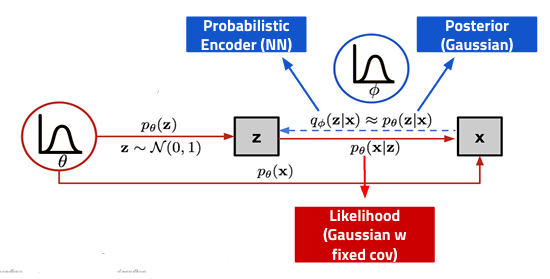
\includegraphics[width=0.75\textwidth]{figuresML_adv/lesson_ml_adv_1_pag_3.png}
\end{center}

Practically speaking, how do we implement this distribution mapping? Instead of a standard Multi-Layer Perceptron (MLP) outputting a single vector $z$, the encoder network $q_\phi$ is designed to output two distinct vectors: a mean ($\mu$) and a standard deviation ($\sigma$). For instance, if we choose a 2-dimensional latent space to easily visualize the data, the network will output two mean values ($\mu_1, \mu_2$) and two standard deviations ($\sigma_1, \sigma_2$). We deliberately assume that the covariance matrix of this multi-dimensional Gaussian is completely diagonal for simplicity. 
Therefore, an input image is no longer encoded as a single dot in the latent space, but rather as a 2D Gaussian curve characterized by the learned $\mu$ and $\sigma$.

To generate the output, we must sample a latent vector $z$ from this newly defined Gaussian distribution and pass it to the decoder. However, this introduces a critical mathematical roadblock during training: the sampling process itself is fundamentally stochastic, meaning it has no derivative. In other words, $\dfrac{\partial z}{\partial \mu}$ and $\dfrac{\partial z}{\partial \sigma}$ cannot be computed if $\mu$ and $\sigma$ are sampled stochastically. If we cannot compute the derivative of the sampling step, then we cannot backpropagate the error through the network to update the encoder weights $\phi$.

To solve this, we employ a clever mathematical workaround known as the \textbf{reparameterization trick}. Instead of sampling directly from the parameterized Gaussian, we express the latent variable as:
\begin{equation}
    z = \mu_\phi(x) + \sigma_\phi(x) \times \epsilon
\end{equation}
where $\epsilon \sim \mathcal{N}(0, I)$ is a small variation sampled from a standard normal distribution. By doing this, we isolate the stochasticity entirely within the independent variable $\epsilon$ and we get
\begin{equation*}
    \dfrac{\partial z}{\partial \mu_{\phi}}=1 \quad, \quad \dfrac{\partial z}{\partial \sigma_{\phi}}=\epsilon
\end{equation*}
The nodes computing $\mu$ and $\sigma$ remain deterministic, allowing the gradients to flow smoothly backward through the network during the optimization process.

\subsection{The Evidence Lower Bound (ELBO) and VAE Loss Function}

Because the VAE is a probabilistic model, its objective function requires a paradigm shift: we must rethink the concept of a loss function as the maximization of a likelihood. 

\subsubsection{Loss Functional as a Likelihood}
To understand this connection, let us recall a standard laboratory physics problem: finding the line of best fit $Y = mX + q$. When we perform this fit by minimizing the $\chi^2$, we are implicitly assuming that the probability density function of our experimental events is Gaussian. The likelihood $\mathcal{L}$ of observing all our data points is the product of these individual Gaussian probabilities:
\begin{equation*}
    \mathcal{L} = \prod_i \text{Gauss}(Y_i - (mX_i + q); \sigma_i)
\end{equation*}
To simplify the mathematics, we take the negative logarithm of the likelihood. Because the logarithm of an exponential leaves only the argument, we obtain:
\begin{equation*}
    -\log \mathcal{L} \sim \sum_i \frac{(Y_i - (mX_i + q))^2}{\sigma_i^2} = \chi^2
\end{equation*}
Finding the optimal parameters $m$ and $q$ by minimizing the $\chi^2$ is therefore mathematically identical to maximizing the likelihood of the data.

This exact logic applies to neural networks. Suppose we have a MLP performing a regression task, learning a function $f_\phi(x)$ parameterized by weights $\phi$. If we assume the output follows a Gaussian distribution with a constant variance $\sigma_i^2 = \text{const}$, the negative log-likelihood becomes:
\begin{equation*}
    -\log \mathcal{L} \sim \sum_i (Y_i - f_\phi(X_i))^2
\end{equation*}
This demonstrates that minimizing the MSE is mathematically equivalent to maximizing a Gaussian likelihood. Similarly, if our data follows a Bernoulli distribution (e.g. binary variables where an event either happens or not), taking the negative log-likelihood of the Bernoulli distribution mathematically yields the binary cross-entropy loss (try to prove it on your own). In short: \textit{every loss function is intrinsically a likelihood}.

\subsubsection{Deriving the ELBO}
In a generative model like a VAE, our primary objective is to maximize the true likelihood of the data, $p_\theta(x)$. However, the true posterior $p_\theta(z|x) = \frac{p_\theta(x,z)}{p_\theta(x)}$ is computationally intractable because calculating $p_\theta(x)$ requires an impossible integration over all possible latent spaces.

To bypass this, we can use a simple but clever trick. We approximate the true posterior using our encoder $q_\phi(z|x)$, and measure the difference between our approximation and the truth using the Kullback-Leibler divergence in eq. \ref{eq:KL_div}, which by definition is always non-negative:
\begin{equation*}
    D_{KL}(q_\phi(z|x) || p_\theta(z|x)) \ge 0
\end{equation*}
Using Bayes' rule, we can substitute $\log p_\theta(z|x) = \log p_\theta(x,z) - \log p_\theta(x)$ into the definition of the KL divergence:
\begin{equation*}
\begin{aligned}
    0 &\le \mathbb{E}_{q_\phi} [\log q_\phi(z|x) - \log p_\theta(z|x)] \quad \Rightarrow \\
    0 &\le \mathbb{E}_{q_\phi} [\log q_\phi(z|x) - (\log p_\theta(x,z) - \log p_\theta(x))] 
\end{aligned}
\end{equation*}
Because $\log p_\theta(x)$ does not depend on the latent variable $z$, we can extract it directly from the expectation. Rearranging the terms, we arrive at a fundamental inequality:
\begin{equation*}
\begin{aligned}
    0 &\le \mathbb{E}_{q_\phi} [\log q_\phi(z|x) - \log p_\theta(x,z)] + \log p_\theta(x) \quad \Rightarrow \\
    \log p_\theta(x) &\ge \mathbb{E}_{q_\phi} [\log p_\theta(x,z) - \log q_\phi(z|x)] \equiv \text{ELBO}
\end{aligned}
\end{equation*}
This term is called the \textbf{Evidence Lower Bound (ELBO)}. Since we cannot maximize the true log-likelihood directly, we maximize the ELBO instead. Pushing up this lower bound guarantees that we are simultaneously pushing up the true likelihood of our data.

By applying the joint probability identity $\log p_\theta(x,z) = \log p_\theta(x|z) + \log p(z)$, we can expand the ELBO into two highly practical terms:
\begin{equation*}
\begin{aligned}
    \text{ELBO} &= \mathbb{E}_{q_\phi} [\log p_\theta(x|z) + \log p(z) - \log q_\phi(z|x)] \quad \Rightarrow \\
    \text{ELBO} &= \mathbb{E}_{q_\phi} [\log p_\theta(x|z)] - D_{KL}(q_\phi(z|x) || p(z))
\end{aligned}
\end{equation*}
Because standard machine learning optimization minimizes a loss function rather than maximizing an objective, the \textbf{VAE Loss Function} is defined as the negative ELBO:
\begin{equation}
    \mathcal{L}_{VAE}(\theta, \phi; x) = - \mathbb{E}_{q_\phi(z|x)}[\log p_\theta(x|z)] + D_{KL}(q_\phi(z|x) || p(z))
\end{equation}

\subsubsection*{Analyzing the Loss Components}
This loss function elegantly balances two competing forces:

\begin{itemize}
    \item \underline{The reconstruction term}: $- \mathbb{E}_{q_\phi}[\log p_\theta(x|z)]$ \\ This is the negative log-likelihood of our decoder. It heavily penalizes the network if it fails to accurately reconstruct the input $x$ from the sampled latent vector $z$. Following our initial digression, we can formally derive the loss based on the data type:
    \begin{itemize}
        \item For continuous data, we assume a \textit{Gaussian} likelihood. The expression mathematically resolves to the MSE:
        \begin{equation*}
        \begin{aligned}
            p_\theta(x|z) &= \mathcal{N}(x; \hat{x}(z), \sigma^2 I) \quad \Rightarrow \\
            -\log p_\theta(x|z) &= \frac{1}{2\sigma^2} ||x - \hat{x}(z)||^2 + \text{const}
        \end{aligned}
        \end{equation*}
        
        \item For binary data (like MNIST pixels), we assume a \textit{Bernoulli} likelihood. The expression mathematically resolves to the BCE:
        \begin{equation*}
        \begin{aligned}
            p_\theta(x|z) &= \text{Bernoulli}(\hat{x}(z)) \quad \Rightarrow \\
            -\log p_\theta(x|z) &= -\sum_{i=1}^{D} [x_i \log \hat{x}_i + (1 - x_i) \log(1 - \hat{x}_i)]
        \end{aligned}
        \end{equation*}
    \end{itemize}
    
    \item \underline {The KL divergence term}: $D_{KL}(q_\phi(z|x) || p(z))$ \\ This term acts as a spatial regularizer. Geometrically, without this term, the network would map different input classes into distant, isolated clusters in the latent space. Sampling from the empty space between these clusters would produce nonsensical noise. The KL divergence acts like a physical spring, pulling the approximate posterior $q_\phi(z|x)$ toward the standard normal prior $p(z) = \mathcal{N}(0, I)$, forcing the clusters to overlap smoothly and creating a continuous generative space.
    
    Because we explicitly defined both the encoder and the prior as Gaussians, this term is not estimated but can be calculated analytically in a closed form. Let the encoder output be $q(z) = \mathcal{N}(z; \mu, \text{diag}(\sigma^2))$ and the prior be $p(z) = \mathcal{N}(z; 0, I)$. Expanding their log-densities yields:
    \begin{equation*}
    \begin{aligned}
        \log q(z) &= -\frac{1}{2}\sum_{j=1}^{d}\left[\log(2\pi\sigma_j^2) + \frac{(z_j-\mu_j)^2}{\sigma_j^2}\right] \\
        \log p(z) &= -\frac{1}{2}\sum_{j=1}^{d}\left[\log(2\pi) + z_j^2\right]
    \end{aligned}
    \end{equation*}
    By substituting these into the definition $D_{KL}(q||p) = \mathbb{E}_{q}[\log q(z) - \log p(z)]$ and evaluating the expectations (knowing that $\mathbb{E}_q[(z_j-\mu_j)^2] = \sigma_j^2$ and $\mathbb{E}_q[z_j^2] = \mu_j^2 + \sigma_j^2$), all constants cancel out beautifully to leave:
    \begin{equation}
        D_{KL}(q||p) = \frac{1}{2} \sum_{j=1}^{d} \left( \mu_j^2 + \sigma_j^2 - 1 - \log \sigma_j^2 \right)
    \end{equation}
\end{itemize}

\subsection{Advanced hands-on example on VAE}
In the following example, a Variational Autoencoder is used to classify user generated images containing rectangles and circles. Instead of using \texttt{keras}, we will be working with the \texttt{PyTorch} module.
The rationale behind this shift is flexibility: especially within the high energy physics community, researchers frequently need to build custom architectures that deviate from standard, built-in models. PyTorch offers the granular control required to implement these novel, physics-informed architectures, making it the standard tool for professional applications. You will find the necessary documentation here: \url{https://docs.pytorch.org/docs/main/}. 

Since I have to start a new page in order to input the Notebook in my LaTeX file, here is a Federer forehand at the 2006 US Open to occupy the rest of the page.

\begin{center}
    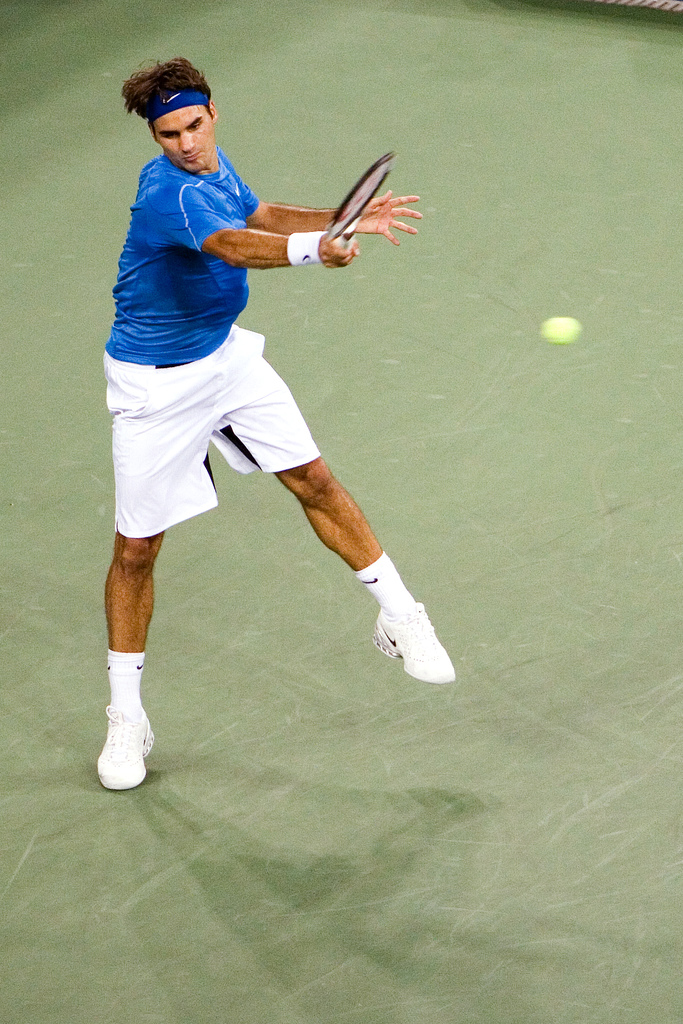
\includegraphics[width=0.25\textwidth]{figuresML/Roger_Federer_US_Open_2006.jpg}
\end{center}

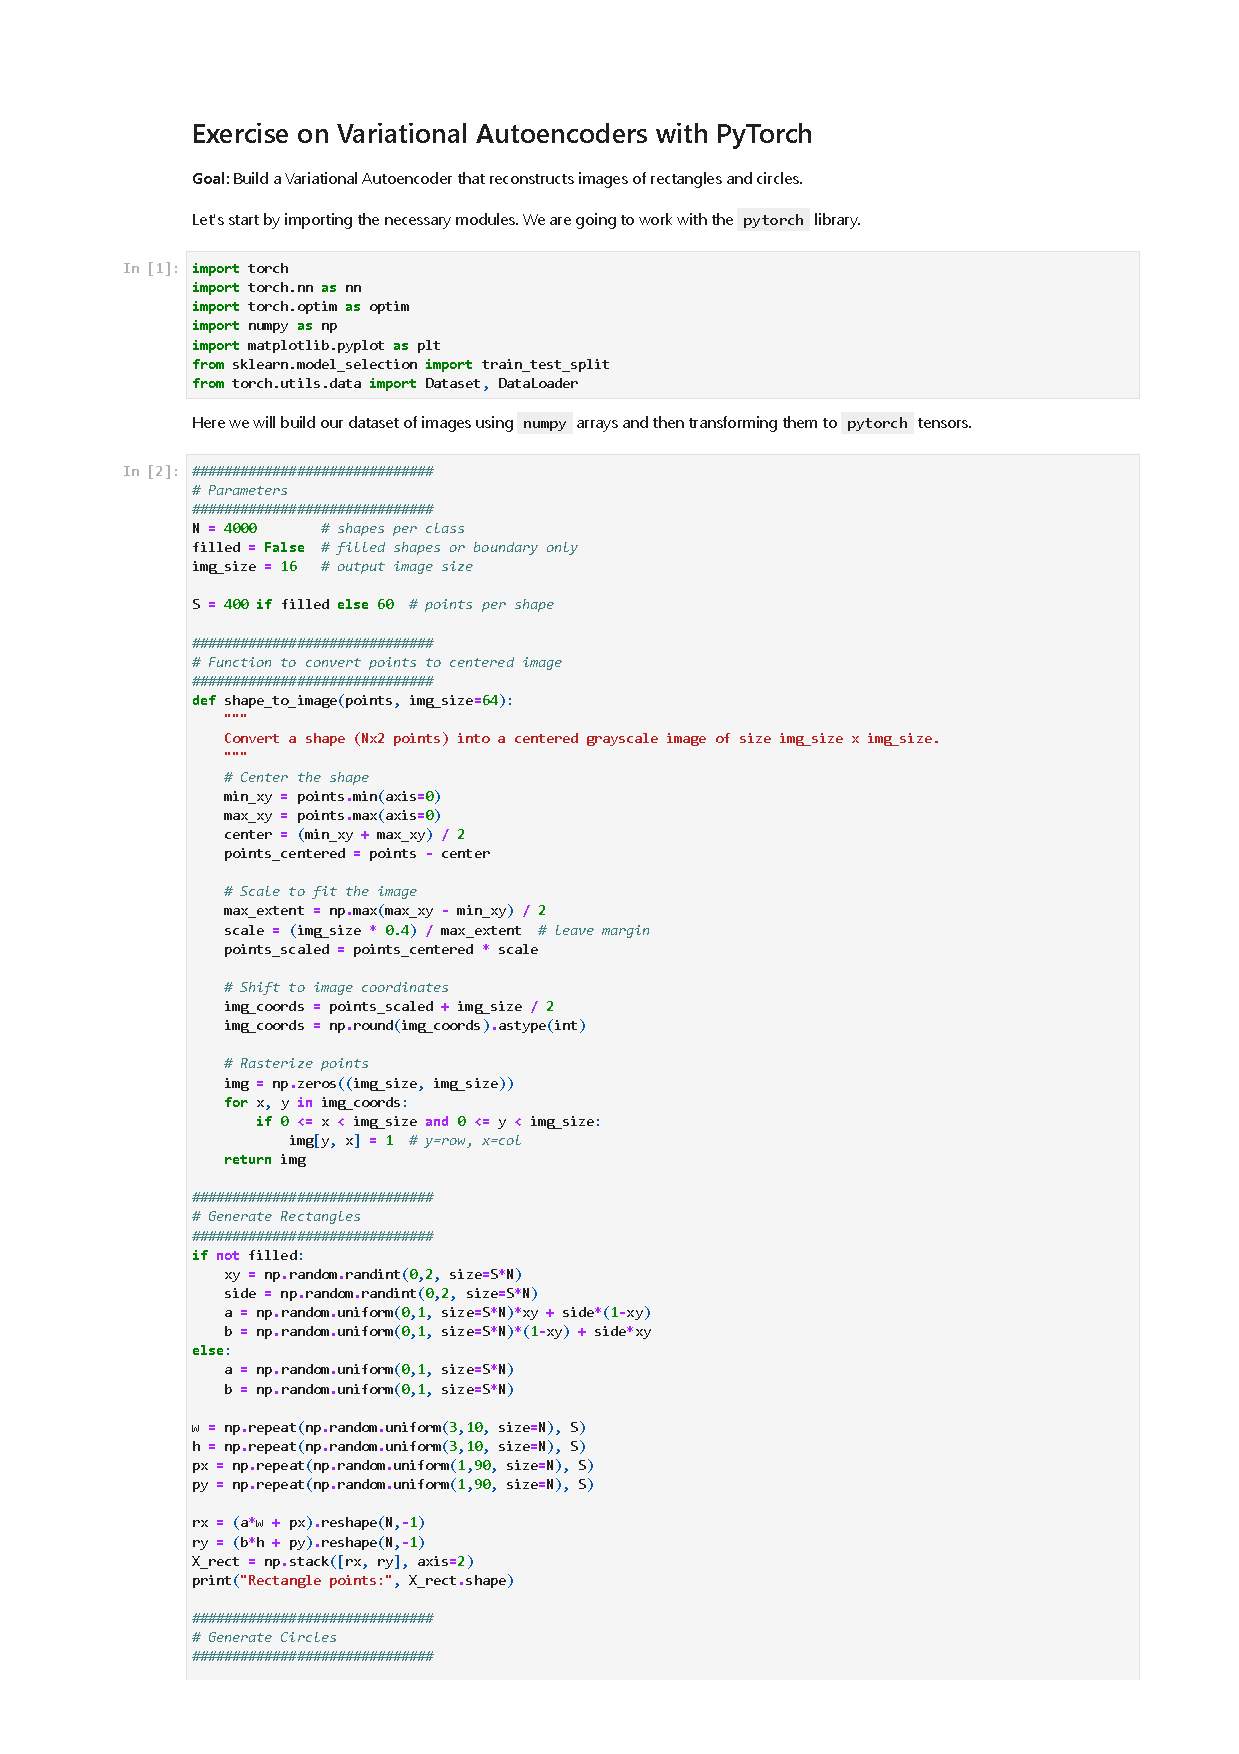
\includepdf[pages=-, pagecommand={\thispagestyle{plain}}]{lezioni/e_ML_adv_1hands_on.pdf} 
% ML_6 nel mio Colab